\documentclass{article} % For LaTeX2e
\usepackage{iclr2021_conference,times}
\usepackage{helvet}
\usepackage{courier}


%\usepackage{subcaption}

\usepackage{amsmath}
\usepackage{amsfonts}
\usepackage[utf8]{inputenc}
\usepackage{amsmath,amssymb}
\usepackage{array}
\usepackage{graphicx}
\usepackage{multirow}
\usepackage{subfig}
\usepackage{todonotes}
\usepackage{listings}
\usepackage{subfigure}
\usepackage{makecell}
\usepackage{times}
\usepackage{helvet}
\usepackage{courier}
\usepackage{algorithm2e}
\RestyleAlgo{ruled}
\usepackage{xcolor}
\usepackage{subfigure}
\usepackage{lipsum} % for filler text


\definecolor{codegreen}{rgb}{0,0.6,0}
\definecolor{codegray}{rgb}{0.5,0.5,0.5}
\definecolor{codepurple}{rgb}{0.58,0,0.82}
\definecolor{backcolour}{rgb}{0.95,0.95,0.92}
% \usepackage[table,xcdraw]{xcolor}
\lstdefinestyle{mystyle}{
    backgroundcolor=\color{backcolour},   
    commentstyle=\color{codegreen},
    keywordstyle=\color{magenta},
    numberstyle=\tiny\color{codegray},
    stringstyle=\color{codepurple},
    basicstyle=\ttfamily\footnotesize,
    breakatwhitespace=false,         
    breaklines=true,                 
    captionpos=b,                    
    keepspaces=true,                 
    numbers=left,                    
    numbersep=5pt,                  
    showspaces=false,                
    showstringspaces=false,
    showtabs=false,                  
    tabsize=2,
    language = python
}

\lstset{style=mystyle}

% Optional math commands from https://github.com/goodfeli/dlbook_notation.
%%%%%% NEW MATH DEFINITIONS %%%%%

\usepackage{amsmath,amsfonts,bm}

% Mark sections of captions for referring to divisions of figures
\newcommand{\figleft}{{\em (Left)}}
\newcommand{\figcenter}{{\em (Center)}}
\newcommand{\figright}{{\em (Right)}}
\newcommand{\figtop}{{\em (Top)}}
\newcommand{\figbottom}{{\em (Bottom)}}
\newcommand{\captiona}{{\em (a)}}
\newcommand{\captionb}{{\em (b)}}
\newcommand{\captionc}{{\em (c)}}
\newcommand{\captiond}{{\em (d)}}

% Highlight a newly defined term
\newcommand{\newterm}[1]{{\bf #1}}


% Figure reference, lower-case.
\def\figref#1{figure~\ref{#1}}
% Figure reference, capital. For start of sentence
\def\Figref#1{Figure~\ref{#1}}
\def\twofigref#1#2{figures \ref{#1} and \ref{#2}}
\def\quadfigref#1#2#3#4{figures \ref{#1}, \ref{#2}, \ref{#3} and \ref{#4}}
% Section reference, lower-case.
\def\secref#1{section~\ref{#1}}
% Section reference, capital.
\def\Secref#1{Section~\ref{#1}}
% Reference to two sections.
\def\twosecrefs#1#2{sections \ref{#1} and \ref{#2}}
% Reference to three sections.
\def\secrefs#1#2#3{sections \ref{#1}, \ref{#2} and \ref{#3}}
% Reference to an equation, lower-case.
\def\eqref#1{equation~\ref{#1}}
% Reference to an equation, upper case
\def\Eqref#1{Equation~\ref{#1}}
% A raw reference to an equation---avoid using if possible
\def\plaineqref#1{\ref{#1}}
% Reference to a chapter, lower-case.
\def\chapref#1{chapter~\ref{#1}}
% Reference to an equation, upper case.
\def\Chapref#1{Chapter~\ref{#1}}
% Reference to a range of chapters
\def\rangechapref#1#2{chapters\ref{#1}--\ref{#2}}
% Reference to an algorithm, lower-case.
\def\algref#1{algorithm~\ref{#1}}
% Reference to an algorithm, upper case.
\def\Algref#1{Algorithm~\ref{#1}}
\def\twoalgref#1#2{algorithms \ref{#1} and \ref{#2}}
\def\Twoalgref#1#2{Algorithms \ref{#1} and \ref{#2}}
% Reference to a part, lower case
\def\partref#1{part~\ref{#1}}
% Reference to a part, upper case
\def\Partref#1{Part~\ref{#1}}
\def\twopartref#1#2{parts \ref{#1} and \ref{#2}}

\def\ceil#1{\lceil #1 \rceil}
\def\floor#1{\lfloor #1 \rfloor}
\def\1{\bm{1}}
\newcommand{\train}{\mathcal{D}}
\newcommand{\valid}{\mathcal{D_{\mathrm{valid}}}}
\newcommand{\test}{\mathcal{D_{\mathrm{test}}}}

\def\eps{{\epsilon}}


% Random variables
\def\reta{{\textnormal{$\eta$}}}
\def\ra{{\textnormal{a}}}
\def\rb{{\textnormal{b}}}
\def\rc{{\textnormal{c}}}
\def\rd{{\textnormal{d}}}
\def\re{{\textnormal{e}}}
\def\rf{{\textnormal{f}}}
\def\rg{{\textnormal{g}}}
\def\rh{{\textnormal{h}}}
\def\ri{{\textnormal{i}}}
\def\rj{{\textnormal{j}}}
\def\rk{{\textnormal{k}}}
\def\rl{{\textnormal{l}}}
% rm is already a command, just don't name any random variables m
\def\rn{{\textnormal{n}}}
\def\ro{{\textnormal{o}}}
\def\rp{{\textnormal{p}}}
\def\rq{{\textnormal{q}}}
\def\rr{{\textnormal{r}}}
\def\rs{{\textnormal{s}}}
\def\rt{{\textnormal{t}}}
\def\ru{{\textnormal{u}}}
\def\rv{{\textnormal{v}}}
\def\rw{{\textnormal{w}}}
\def\rx{{\textnormal{x}}}
\def\ry{{\textnormal{y}}}
\def\rz{{\textnormal{z}}}

% Random vectors
\def\rvepsilon{{\mathbf{\epsilon}}}
\def\rvtheta{{\mathbf{\theta}}}
\def\rva{{\mathbf{a}}}
\def\rvb{{\mathbf{b}}}
\def\rvc{{\mathbf{c}}}
\def\rvd{{\mathbf{d}}}
\def\rve{{\mathbf{e}}}
\def\rvf{{\mathbf{f}}}
\def\rvg{{\mathbf{g}}}
\def\rvh{{\mathbf{h}}}
\def\rvu{{\mathbf{i}}}
\def\rvj{{\mathbf{j}}}
\def\rvk{{\mathbf{k}}}
\def\rvl{{\mathbf{l}}}
\def\rvm{{\mathbf{m}}}
\def\rvn{{\mathbf{n}}}
\def\rvo{{\mathbf{o}}}
\def\rvp{{\mathbf{p}}}
\def\rvq{{\mathbf{q}}}
\def\rvr{{\mathbf{r}}}
\def\rvs{{\mathbf{s}}}
\def\rvt{{\mathbf{t}}}
\def\rvu{{\mathbf{u}}}
\def\rvv{{\mathbf{v}}}
\def\rvw{{\mathbf{w}}}
\def\rvx{{\mathbf{x}}}
\def\rvy{{\mathbf{y}}}
\def\rvz{{\mathbf{z}}}

% Elements of random vectors
\def\erva{{\textnormal{a}}}
\def\ervb{{\textnormal{b}}}
\def\ervc{{\textnormal{c}}}
\def\ervd{{\textnormal{d}}}
\def\erve{{\textnormal{e}}}
\def\ervf{{\textnormal{f}}}
\def\ervg{{\textnormal{g}}}
\def\ervh{{\textnormal{h}}}
\def\ervi{{\textnormal{i}}}
\def\ervj{{\textnormal{j}}}
\def\ervk{{\textnormal{k}}}
\def\ervl{{\textnormal{l}}}
\def\ervm{{\textnormal{m}}}
\def\ervn{{\textnormal{n}}}
\def\ervo{{\textnormal{o}}}
\def\ervp{{\textnormal{p}}}
\def\ervq{{\textnormal{q}}}
\def\ervr{{\textnormal{r}}}
\def\ervs{{\textnormal{s}}}
\def\ervt{{\textnormal{t}}}
\def\ervu{{\textnormal{u}}}
\def\ervv{{\textnormal{v}}}
\def\ervw{{\textnormal{w}}}
\def\ervx{{\textnormal{x}}}
\def\ervy{{\textnormal{y}}}
\def\ervz{{\textnormal{z}}}

% Random matrices
\def\rmA{{\mathbf{A}}}
\def\rmB{{\mathbf{B}}}
\def\rmC{{\mathbf{C}}}
\def\rmD{{\mathbf{D}}}
\def\rmE{{\mathbf{E}}}
\def\rmF{{\mathbf{F}}}
\def\rmG{{\mathbf{G}}}
\def\rmH{{\mathbf{H}}}
\def\rmI{{\mathbf{I}}}
\def\rmJ{{\mathbf{J}}}
\def\rmK{{\mathbf{K}}}
\def\rmL{{\mathbf{L}}}
\def\rmM{{\mathbf{M}}}
\def\rmN{{\mathbf{N}}}
\def\rmO{{\mathbf{O}}}
\def\rmP{{\mathbf{P}}}
\def\rmQ{{\mathbf{Q}}}
\def\rmR{{\mathbf{R}}}
\def\rmS{{\mathbf{S}}}
\def\rmT{{\mathbf{T}}}
\def\rmU{{\mathbf{U}}}
\def\rmV{{\mathbf{V}}}
\def\rmW{{\mathbf{W}}}
\def\rmX{{\mathbf{X}}}
\def\rmY{{\mathbf{Y}}}
\def\rmZ{{\mathbf{Z}}}

% Elements of random matrices
\def\ermA{{\textnormal{A}}}
\def\ermB{{\textnormal{B}}}
\def\ermC{{\textnormal{C}}}
\def\ermD{{\textnormal{D}}}
\def\ermE{{\textnormal{E}}}
\def\ermF{{\textnormal{F}}}
\def\ermG{{\textnormal{G}}}
\def\ermH{{\textnormal{H}}}
\def\ermI{{\textnormal{I}}}
\def\ermJ{{\textnormal{J}}}
\def\ermK{{\textnormal{K}}}
\def\ermL{{\textnormal{L}}}
\def\ermM{{\textnormal{M}}}
\def\ermN{{\textnormal{N}}}
\def\ermO{{\textnormal{O}}}
\def\ermP{{\textnormal{P}}}
\def\ermQ{{\textnormal{Q}}}
\def\ermR{{\textnormal{R}}}
\def\ermS{{\textnormal{S}}}
\def\ermT{{\textnormal{T}}}
\def\ermU{{\textnormal{U}}}
\def\ermV{{\textnormal{V}}}
\def\ermW{{\textnormal{W}}}
\def\ermX{{\textnormal{X}}}
\def\ermY{{\textnormal{Y}}}
\def\ermZ{{\textnormal{Z}}}

% Vectors
\def\vzero{{\bm{0}}}
\def\vone{{\bm{1}}}
\def\vmu{{\bm{\mu}}}
\def\vtheta{{\bm{\theta}}}
\def\va{{\bm{a}}}
\def\vb{{\bm{b}}}
\def\vc{{\bm{c}}}
\def\vd{{\bm{d}}}
\def\ve{{\bm{e}}}
\def\vf{{\bm{f}}}
\def\vg{{\bm{g}}}
\def\vh{{\bm{h}}}
\def\vi{{\bm{i}}}
\def\vj{{\bm{j}}}
\def\vk{{\bm{k}}}
\def\vl{{\bm{l}}}
\def\vm{{\bm{m}}}
\def\vn{{\bm{n}}}
\def\vo{{\bm{o}}}
\def\vp{{\bm{p}}}
\def\vq{{\bm{q}}}
\def\vr{{\bm{r}}}
\def\vs{{\bm{s}}}
\def\vt{{\bm{t}}}
\def\vu{{\bm{u}}}
\def\vv{{\bm{v}}}
\def\vw{{\bm{w}}}
\def\vx{{\bm{x}}}
\def\vy{{\bm{y}}}
\def\vz{{\bm{z}}}

% Elements of vectors
\def\evalpha{{\alpha}}
\def\evbeta{{\beta}}
\def\evepsilon{{\epsilon}}
\def\evlambda{{\lambda}}
\def\evomega{{\omega}}
\def\evmu{{\mu}}
\def\evpsi{{\psi}}
\def\evsigma{{\sigma}}
\def\evtheta{{\theta}}
\def\eva{{a}}
\def\evb{{b}}
\def\evc{{c}}
\def\evd{{d}}
\def\eve{{e}}
\def\evf{{f}}
\def\evg{{g}}
\def\evh{{h}}
\def\evi{{i}}
\def\evj{{j}}
\def\evk{{k}}
\def\evl{{l}}
\def\evm{{m}}
\def\evn{{n}}
\def\evo{{o}}
\def\evp{{p}}
\def\evq{{q}}
\def\evr{{r}}
\def\evs{{s}}
\def\evt{{t}}
\def\evu{{u}}
\def\evv{{v}}
\def\evw{{w}}
\def\evx{{x}}
\def\evy{{y}}
\def\evz{{z}}

% Matrix
\def\mA{{\bm{A}}}
\def\mB{{\bm{B}}}
\def\mC{{\bm{C}}}
\def\mD{{\bm{D}}}
\def\mE{{\bm{E}}}
\def\mF{{\bm{F}}}
\def\mG{{\bm{G}}}
\def\mH{{\bm{H}}}
\def\mI{{\bm{I}}}
\def\mJ{{\bm{J}}}
\def\mK{{\bm{K}}}
\def\mL{{\bm{L}}}
\def\mM{{\bm{M}}}
\def\mN{{\bm{N}}}
\def\mO{{\bm{O}}}
\def\mP{{\bm{P}}}
\def\mQ{{\bm{Q}}}
\def\mR{{\bm{R}}}
\def\mS{{\bm{S}}}
\def\mT{{\bm{T}}}
\def\mU{{\bm{U}}}
\def\mV{{\bm{V}}}
\def\mW{{\bm{W}}}
\def\mX{{\bm{X}}}
\def\mY{{\bm{Y}}}
\def\mZ{{\bm{Z}}}
\def\mBeta{{\bm{\beta}}}
\def\mPhi{{\bm{\Phi}}}
\def\mLambda{{\bm{\Lambda}}}
\def\mSigma{{\bm{\Sigma}}}

% Tensor
\DeclareMathAlphabet{\mathsfit}{\encodingdefault}{\sfdefault}{m}{sl}
\SetMathAlphabet{\mathsfit}{bold}{\encodingdefault}{\sfdefault}{bx}{n}
\newcommand{\tens}[1]{\bm{\mathsfit{#1}}}
\def\tA{{\tens{A}}}
\def\tB{{\tens{B}}}
\def\tC{{\tens{C}}}
\def\tD{{\tens{D}}}
\def\tE{{\tens{E}}}
\def\tF{{\tens{F}}}
\def\tG{{\tens{G}}}
\def\tH{{\tens{H}}}
\def\tI{{\tens{I}}}
\def\tJ{{\tens{J}}}
\def\tK{{\tens{K}}}
\def\tL{{\tens{L}}}
\def\tM{{\tens{M}}}
\def\tN{{\tens{N}}}
\def\tO{{\tens{O}}}
\def\tP{{\tens{P}}}
\def\tQ{{\tens{Q}}}
\def\tR{{\tens{R}}}
\def\tS{{\tens{S}}}
\def\tT{{\tens{T}}}
\def\tU{{\tens{U}}}
\def\tV{{\tens{V}}}
\def\tW{{\tens{W}}}
\def\tX{{\tens{X}}}
\def\tY{{\tens{Y}}}
\def\tZ{{\tens{Z}}}


% Graph
\def\gA{{\mathcal{A}}}
\def\gB{{\mathcal{B}}}
\def\gC{{\mathcal{C}}}
\def\gD{{\mathcal{D}}}
\def\gE{{\mathcal{E}}}
\def\gF{{\mathcal{F}}}
\def\gG{{\mathcal{G}}}
\def\gH{{\mathcal{H}}}
\def\gI{{\mathcal{I}}}
\def\gJ{{\mathcal{J}}}
\def\gK{{\mathcal{K}}}
\def\gL{{\mathcal{L}}}
\def\gM{{\mathcal{M}}}
\def\gN{{\mathcal{N}}}
\def\gO{{\mathcal{O}}}
\def\gP{{\mathcal{P}}}
\def\gQ{{\mathcal{Q}}}
\def\gR{{\mathcal{R}}}
\def\gS{{\mathcal{S}}}
\def\gT{{\mathcal{T}}}
\def\gU{{\mathcal{U}}}
\def\gV{{\mathcal{V}}}
\def\gW{{\mathcal{W}}}
\def\gX{{\mathcal{X}}}
\def\gY{{\mathcal{Y}}}
\def\gZ{{\mathcal{Z}}}

% Sets
\def\sA{{\mathbb{A}}}
\def\sB{{\mathbb{B}}}
\def\sC{{\mathbb{C}}}
\def\sD{{\mathbb{D}}}
% Don't use a set called E, because this would be the same as our symbol
% for expectation.
\def\sF{{\mathbb{F}}}
\def\sG{{\mathbb{G}}}
\def\sH{{\mathbb{H}}}
\def\sI{{\mathbb{I}}}
\def\sJ{{\mathbb{J}}}
\def\sK{{\mathbb{K}}}
\def\sL{{\mathbb{L}}}
\def\sM{{\mathbb{M}}}
\def\sN{{\mathbb{N}}}
\def\sO{{\mathbb{O}}}
\def\sP{{\mathbb{P}}}
\def\sQ{{\mathbb{Q}}}
\def\sR{{\mathbb{R}}}
\def\sS{{\mathbb{S}}}
\def\sT{{\mathbb{T}}}
\def\sU{{\mathbb{U}}}
\def\sV{{\mathbb{V}}}
\def\sW{{\mathbb{W}}}
\def\sX{{\mathbb{X}}}
\def\sY{{\mathbb{Y}}}
\def\sZ{{\mathbb{Z}}}

% Entries of a matrix
\def\emLambda{{\Lambda}}
\def\emA{{A}}
\def\emB{{B}}
\def\emC{{C}}
\def\emD{{D}}
\def\emE{{E}}
\def\emF{{F}}
\def\emG{{G}}
\def\emH{{H}}
\def\emI{{I}}
\def\emJ{{J}}
\def\emK{{K}}
\def\emL{{L}}
\def\emM{{M}}
\def\emN{{N}}
\def\emO{{O}}
\def\emP{{P}}
\def\emQ{{Q}}
\def\emR{{R}}
\def\emS{{S}}
\def\emT{{T}}
\def\emU{{U}}
\def\emV{{V}}
\def\emW{{W}}
\def\emX{{X}}
\def\emY{{Y}}
\def\emZ{{Z}}
\def\emSigma{{\Sigma}}

% entries of a tensor
% Same font as tensor, without \bm wrapper
\newcommand{\etens}[1]{\mathsfit{#1}}
\def\etLambda{{\etens{\Lambda}}}
\def\etA{{\etens{A}}}
\def\etB{{\etens{B}}}
\def\etC{{\etens{C}}}
\def\etD{{\etens{D}}}
\def\etE{{\etens{E}}}
\def\etF{{\etens{F}}}
\def\etG{{\etens{G}}}
\def\etH{{\etens{H}}}
\def\etI{{\etens{I}}}
\def\etJ{{\etens{J}}}
\def\etK{{\etens{K}}}
\def\etL{{\etens{L}}}
\def\etM{{\etens{M}}}
\def\etN{{\etens{N}}}
\def\etO{{\etens{O}}}
\def\etP{{\etens{P}}}
\def\etQ{{\etens{Q}}}
\def\etR{{\etens{R}}}
\def\etS{{\etens{S}}}
\def\etT{{\etens{T}}}
\def\etU{{\etens{U}}}
\def\etV{{\etens{V}}}
\def\etW{{\etens{W}}}
\def\etX{{\etens{X}}}
\def\etY{{\etens{Y}}}
\def\etZ{{\etens{Z}}}

% The true underlying data generating distribution
\newcommand{\pdata}{p_{\rm{data}}}
% The empirical distribution defined by the training set
\newcommand{\ptrain}{\hat{p}_{\rm{data}}}
\newcommand{\Ptrain}{\hat{P}_{\rm{data}}}
% The model distribution
\newcommand{\pmodel}{p_{\rm{model}}}
\newcommand{\Pmodel}{P_{\rm{model}}}
\newcommand{\ptildemodel}{\tilde{p}_{\rm{model}}}
% Stochastic autoencoder distributions
\newcommand{\pencode}{p_{\rm{encoder}}}
\newcommand{\pdecode}{p_{\rm{decoder}}}
\newcommand{\precons}{p_{\rm{reconstruct}}}

\newcommand{\laplace}{\mathrm{Laplace}} % Laplace distribution

\newcommand{\E}{\mathbb{E}}
\newcommand{\Ls}{\mathcal{L}}
\newcommand{\R}{\mathbb{R}}
\newcommand{\emp}{\tilde{p}}
\newcommand{\lr}{\alpha}
\newcommand{\reg}{\lambda}
\newcommand{\rect}{\mathrm{rectifier}}
\newcommand{\softmax}{\mathrm{softmax}}
\newcommand{\sigmoid}{\sigma}
\newcommand{\softplus}{\zeta}
\newcommand{\KL}{D_{\mathrm{KL}}}
\newcommand{\Var}{\mathrm{Var}}
\newcommand{\standarderror}{\mathrm{SE}}
\newcommand{\Cov}{\mathrm{Cov}}
% Wolfram Mathworld says $L^2$ is for function spaces and $\ell^2$ is for vectors
% But then they seem to use $L^2$ for vectors throughout the site, and so does
% wikipedia.
\newcommand{\normlzero}{L^0}
\newcommand{\normlone}{L^1}
\newcommand{\normltwo}{L^2}
\newcommand{\normlp}{L^p}
\newcommand{\normmax}{L^\infty}

\newcommand{\parents}{Pa} % See usage in notation.tex. Chosen to match Daphne's book.

\DeclareMathOperator*{\argmax}{arg\,max}
\DeclareMathOperator*{\argmin}{arg\,min}

\DeclareMathOperator{\sign}{sign}
\DeclareMathOperator{\Tr}{Tr}
\let\ab\allowbreak


\usepackage{hyperref}
\usepackage{url}


\title{Leveraging Large Language Models for Creative Story Generation}

% Authors must not appear in the submitted version. They should be hidden
% as long as the \iclrfinalcopy macro remains commented out below.
% Non-anonymous submissions will be rejected without review.

\author{Yuetian Chen, and Brendan Capuzzo \\
Group U1 - Machine Learning and Optimization \\
CSCI 4968 - 01 - Spring 2023\\
Department of Computer Science\\
Rensselaer Polytechnic Institute\\
Troy, NY 12180, USA \\
\texttt{\{cheny63, capuzb\}@rpi.edu} \\
% \And
% Ji Q. Ren \& Yevgeny LeNet \\
% Department of Computational Neuroscience \\
% University of the Witwatersrand \\
% Joburg, South Africa \\
% \texttt{\{robot,net\}@wits.ac.za} \\
% \AND
% Coauthor \\
% Affiliation \\
% Address \\
% \texttt{email}
}

% The \author macro works with any number of authors. There are two commands
% used to separate the names and addresses of multiple authors: \And and \AND.
%
% Using \And between authors leaves it to \LaTeX{} to determine where to break
% the lines. Using \AND forces a linebreak at that point. So, if \LaTeX{}
% puts 3 of 4 authors names on the first line, and the last on the second
% line, try using \AND instead of \And before the third author name.

\newcommand{\fix}{\marginpar{FIX}}
\newcommand{\new}{\marginpar{NEW}}

\iclrfinalcopy % Uncomment for camera-ready version, but NOT for submission.
\begin{document}


\maketitle

\begin{abstract}
Creative story generation is a challenging and intriguing task in the field of natural language processing. With the advent of Large Language Models (LLMs), there is growing interest in utilizing their impressive text generation capabilities for generating coherent and engaging stories. In this paper, we investigate the potential of Large Language Models (LLMs) for creative story generation, aiming to develop a framework that generates coherent and engaging stories characterized by rich narrative structures. Our methodology combines LLM fine-tuning with knowledge distillation techniques, utilizing both teacher and student models to create a computationally efficient framework capable of producing captivating stories without compromising text quality. We provide an in-depth overview of our methodology, detailing the implementation of knowledge distillation and its associated loss functions. Our experiments demonstrate the effectiveness of our proposed framework in generating creative stories, offering valuable insights for future research in this domain. Additionally, we identify potential areas for future work, including the exploration of alternative divergence measures and the investigation of self-distillation for language generation. This research contributes to the growing body of work on LLMs and their applications in creative storytelling, paving the way for more advanced and efficient story generation systems.\footnote{GitHub Repository: \hyperref[https://github.com/Stry233/MlAndOpt-LLM-for-Creative-Story-Generation]{https://github.com/Stry233/MlAndOpt-LLM-for-Creative-Story-Generation}}\footnote{Demo link: \hyperref[http://vsg-ek.herokuapp.com/]{http://vsg-ek.herokuapp.com/}}
\end{abstract}

\section{Introduction}

Storytelling is a fundamental aspect of human culture, allowing us to communicate, entertain, and educate. With the advent of artificial intelligence and natural language processing, the possibility of generating creative and engaging stories automatically has become an exciting research area. Large Language Models (LLMs), such as GPT-3~\cite{brown2020language} and T5, have demonstrated impressive capabilities in generating human-like text, making them promising candidates for creative story generation.

In this report, we detail our research project, which focuses on investigating the potential of LLMs for creative story generation. Our primary objective is to improve the framework that leverages the text generation capabilities of LLMs and combines them with novel techniques for narrative structure generation. This would allow the generation of coherent and engaging stories that encompass rich narrative structures, including character development, plot progression, and conflict resolution. As shown in Table~\ref{storyExampleII}, for language models with fewer parameters, this is never an easy task.

\begin{table}[h]
    \centering
    \caption{An example comparing the results generated from our framework (\textbf{expected}) and baseline model (\textbf{actual [Zero-shot \texttt{T5$_{base}$}]})}
    \begin{tabular}{p{0.01\linewidth} | p{0.40\linewidth}|p{0.40\linewidth}}
    \textbf{\#} & \textbf{expected}                & \textbf{actual [Zero-shot \texttt{T5$_{base}$}]}                \\ \hline
    1 & Mary had been feeling depressed lately.                        & Mary had been feeling depressed lately. \\ \hline
    2 & she decided to go see a psychiatrist.                          & She decided to go to a psychiatrist.    \\ \hline
    3 & Psyched, her psychiatrist diagnosed her with depression and sent her to see. & She was diagnosed with schizophrenia. \\ \hline
    4 & Medicant took her to get an antidepressant and prescribed her. & She was very happy.                     \\ \hline
    5 & Thankfully it eventually made her feel better again.           & She was very happy.                    
    \end{tabular}%
    \label{storyExampleII}
\end{table}

To achieve this goal, we have been working on several tasks, including understanding the current state of the art in story generation, analyzing the strengths and limitations of existing LLMs, and exploring various techniques for generating narrative structures. In the following sections, we will discuss our methodology, preliminary work, and the progress we have made in our project as well as related work.


\section{Related Work}
\subsection{Visual Story Generation}
Storytelling is an important part of human lives and can be portrayed in numerous means. Stories can be conveyed through text or they can incorporate visual aspects. Visual storytelling helps to provide more detail and engagement to stories. While large language models have performed exceedingly well on text generation, recent research such as ~\cite{Chen_Li_Shi_Liu_Si_2023} has been utilizing these large language models to co-create visual stories. Visual story generation is often aided by user input or control to provide suggestions for how the visual stories should be developed. Objects and locations are utilized to generate visuals for text-generated sentences. These visualizations use image/object recognition to ensure that visuals accurately depict the text-based story.

\subsection{Text Generation Control}
While text generation has been extremely powerful and successful in the last decade with recent developments such as GPT-3, many models have lacked the element of control. Recent research such as ~\cite{Yu_Yu_Sagae_2021}, has introduced methods such as attribute alignment, which utilizes an attribute function to guide a pre-trained language model without changing parameters. This method uses emotions and topics as indicators for controlling text generation. Essentially, given a prompt, the next generated sentence will relate to the "attribute" that is assigned, such as a topic (i.e. politics, sports, etc.). This allows the generated text to be fine-tuned to produce specialized results. The field of control over text generation is an emerging area of research as large language models have been deployed for public use.

\subsection{Automatic Storytelling}
Automatic story generation has long been a challenging task in natural language processing, and such efforts date back to the 1970s~\cite{Meehan1977TALESPINAI}. Earlier attempts, such as symbolic planning systems~\cite{Riedl_2010}, utilize planning techniques to create plausible and coherent plots for stories. In addition, case-based or analogical modeling systems generate new narratives based on adapted existing stories~\cite{Gervs2005StoryPG}. However, while these approaches can create stories with impressive coherence and consistency, they often require extensive knowledge engineering and restrict to a limited domain. To address the issue, large crowd-sourced corpora of stories are used to help generate stories~\cite{10.1145/2362394.2362398,Li}. Modern approaches based on neural language models have been explored to generate plot-driven stories~\cite{fan-etal-2018-hierarchical}. Moreover,~\cite{yang-etal-2019-enhancing-topic} incorporates commonsense knowledge into the generator using a novel memory mechanism and utilizes adversarial training to improve the diversity and originality of essay generation.~\cite{Tambwekar2019ControllableNS} leverages reward strategies during the generation to guide the language model toward generating a coherent story.~\cite{Liu_Li_Yu_Huang_Liu_Zhao_Yan_2020} proposes a character-centric story-generation model that can produce stories consistent with characters' profiles. 

\subsection{Commonsense Reasoning}
In hopes of leveraging large language models to become ``smarter" and more responsive text generation tools, many people have dedicated research towards improving the reasoning skills of these models. The research in ~\cite{Lin_Zhou_Shen_Zhou_Bhagavatula_Choi_Ren_2020} talks about utilizing a commonGen ~\cite{lin2020commongen} dataset which contains concept sets of objects and actions that relate to each other as well as example sentences featuring these sets. The focus behind using this dataset is to improve the reasoning and ability to make decisions based on common sense when generating text. The goal is to teach models to understand how words and concepts are used together and be able to recognize these concepts. This research is further analyzed in ~\cite{Chen_Chen_Yu_2018} with a focus on story generation. This research helps to train models to dynamically complete generated stories based on knowledge from the CommonGen\cite{lin2019commongen} dataset. By knowing how a set of words is related, the large language model is better able to choose and predict the next sentence in a story.

\subsection{Knowledge Distillation for Language Generation}
Knowledge distillation is a technique that involves transferring knowledge from a larger, more complex model (teacher model) to a smaller, more efficient model (student model) \cite{Huang_2021_CVPR}. This process allows the student model to benefit from the knowledge and generalization ability of the teacher model while having a smaller model size and faster inference time. In recent years, knowledge distillation has been applied to various tasks in natural language processing, including language generation \cite{kim2016sequencelevel, 10.1145/1150402.1150464}. This technique has shown great promise in reducing the computational cost of large language models while maintaining their powerful text generation capabilities. 

For instance, \cite{Sanh2020DistilBERTAD} introduces DistilBERT, a smaller version of BERT \cite{devlin2018bert} obtained through knowledge distillation. DistilBERT retains most of the original BERT's capabilities while being significantly smaller in size and faster in inference time. Similarly, \cite{tang-etal-2019-natural} presents a method for distilling the knowledge of GPT-3 into a smaller model. By carefully designing the training objective and data selection, they demonstrate that the distilled model can achieve competitive performance with the original GPT-3 model on various benchmarks while having a smaller model size. 

In our work, we take inspiration from these knowledge distillation techniques and apply them to our interactive visual story generation pipeline. By incorporating a distilled language model into our system, we aim to maintain the powerful text generation capabilities of the large language model while ensuring a more efficient and computationally feasible solution for real-time user interaction.


\section{Methodology}
In this section, we provide an in-depth overview of the methodology utilized in our research project, which focuses on creative story generation using Large Language Models (LLMs) such as T5. Our approach is built on a foundation of two key components: LLM fine-tuning, and knowledge distillation. These components work in tandem to create a comprehensive framework that generates engaging stories with rich narrative structures.

% \textbf{LLM Fine-tuning:} The first component of our methodology involves fine-tuning pre-trained LLMs on a dataset specifically created for the purpose of creative story generation. This dataset includes a diverse selection of high-quality stories, covering a wide range of themes, genres, and narrative styles. The fine-tuning process enables the LLM to learn the nuances of creative storytelling, including character development, plot progression, and conflict resolution. By adjusting the model's parameters and employing various optimization techniques, we aim to maximize the performance of the fine-tuned model in generating creative stories.
\subsection{Fine-Tuning Pre-trained Language Models for Content Generation}
The first component of our methodology involves fine-tuning pre-trained Language Models (LLMs) on a dataset specifically created for the purpose of creative story generation. This dataset includes a diverse selection of high-quality stories, covering a wide range of themes, genres, and narrative styles. The fine-tuning process enables the LLM to learn the nuances of creative storytelling, including character development, plot progression, and conflict resolution. By adjusting the model's parameters and employing various optimization techniques, we aim to maximize the performance of the fine-tuned model in generating creative stories.
Given the dataset $D$, the objective of the fine-tuning process is to adjust the parameters of the pre-trained LLM, $\theta$, to minimize the cross-entropy loss between the model's output probabilities and the true token labels.
\begin{figure}
    \centering
    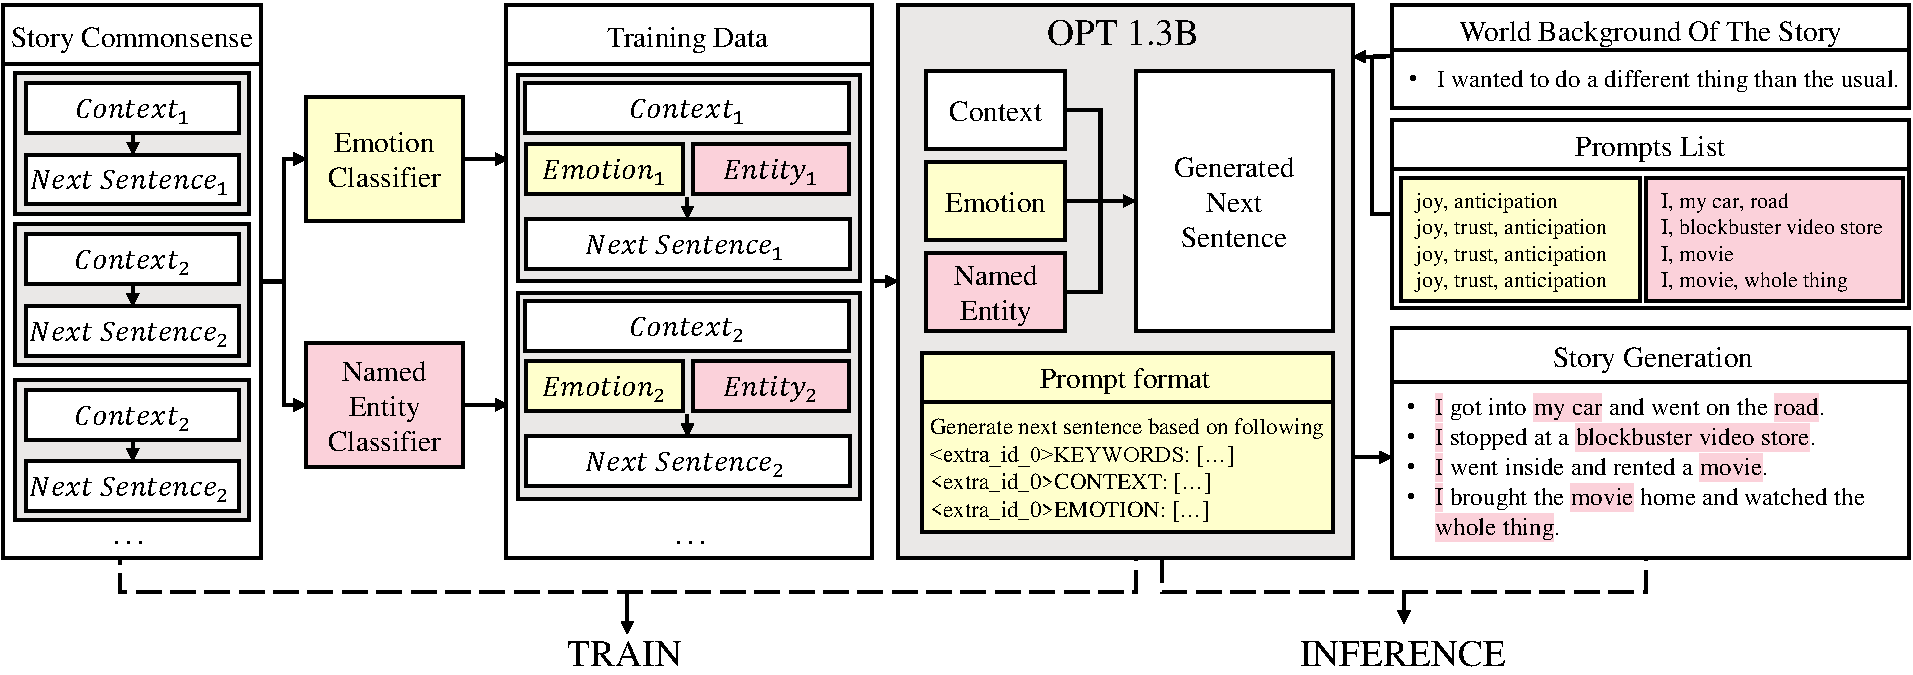
\includegraphics[width=\linewidth]{figure/pipe.pdf}
    \caption{Optimized training and inference pipeline for Next Sentence Generation.}
    \label{fig:pipe}
\end{figure}

\begin{equation}
\mathcal{L}_{FT}(\theta) = - \sum_{i=1}^N \sum_{t=1}^{T^{(i)}} \log P_\theta(y_t^{(i)} | x^{(i)})
\end{equation}

As shown in Algorithm 1, $T^{(i)}$ is the length of the target sequence $y^{(i)}$, and $P_\theta(y_t^{(i)} | x^{(i)})$ is the probability of the true token $y_t^{(i)}$ at position $t$ given the input sequence $x^{(i)}$ and the model parameters $\theta$. We fine-tune the pre-trained LLM using the collected dataset and the optimization techniques mentioned above. The training process is illustrated in the following pseudo-code:

\SetKwComment{Comment}{/* }{ */}
\begin{algorithm}
    \caption{Fine-Tuning Pre-trained Language Models for Creative Story Generation}\label{alg:fine-tuning}
    \KwData{Dataset $D = \{(x^{(i)}, y^{(i)})\}_{i=1}^N$, pre-trained LLM with parameters $\theta$, optimization method, learning rate schedule, and other hyperparameters}
    \KwResult{Fine-tuned LLM with parameters $\theta'$}
    Initialize the pre-trained LLM with parameters $\theta$\;
    Set the learning rate schedule, optimization method, and other hyperparameters\;
    \For{epoch $= 1$ \KwTo num\_epochs}{
      Shuffle the dataset $D$\;
      \For{each mini-batch $(x_{\text{batch}}, y_{\text{batch}})$ in $D$}{
        Compute the gradients of the loss function $\mathcal{L}_{FT}(\theta)$ with respect to $\theta$\;
        Update the model parameters $\theta$ using the gradients and the optimization method\;
        Clip the gradients if necessary\Comment*[r]{Gradient clipping}\\
        Apply dropout for regularization\;
      }
    }
    Save the fine-tuned model with parameters $\theta'$\;
\end{algorithm}

An overview of our model finetuning procedure is given in Figure~\ref{fig:pipe}. For a sample story $\vec{D} \in \mathbf{D}$, we define it as a 5-dimensional vector $\vec{D} = \{d_1, \dots, d_5\}$ where each $d_i$ represents the corresponding sentence in the story. % To encourage the model to understand the propulsive nature of the storyline and the pattern of story development at $i^{\text{th}}$ stages, $\vec{S}$ needs to be further partitioned into $\vec{S_1}, \dots, \vec{S_5}$ such that:
%
%So far, we have obtained the contextual content of each story from $\mathbf{S_{total}}$ when it is about to move to the next stage $s_{j+1}$ (which is also the entry our story generation model will generate). 

For training our system to generate the next sentence, $d_{j+1}$ is fed into the emotion classifier as well as the keyword extractor for identifying the emotions and keywords in the next sentence. Based on story context and the additional knowledge input, the language model is trained on a triad of data: context, keyword, and emotion labels. 

In addition, we used the following prompting structure in both the training as well as inference processes:
\begin{lstlisting}
Generate next sentence based on following 
<extra_id_0>KEYWORDS: [...]
<extra_id_0>CONTEXT: [...]
<extra_id_0>EMOTION: [...]
\end{lstlisting}

By fine-tuning \texttt{OPT 1.3b} based on the emotions and the keyword information as prompts, the model can more effectively capture hidden information in the story and thus improve the accuracy and variety of sentences, which can serve as the teacher network in the following procedure.


\subsection{Knowledge Distillation}
Knowledge distillation is a technique used to transfer knowledge from a large, pre-trained teacher model to a smaller student model. In this section, we describe in detail the implementation of knowledge distillation for language generation using the provided code snippet. In this section, we have detailed the implementation of knowledge distillation for language generation using a teacher model and a student model. We discussed the equations, objective/loss function, and necessary derivations for this implementation. The main steps of the implementation are:
\begin{itemize}
    \item Selecting teacher and student model architectures
    \item Tokenizing and batching input text data
    \item Generating soft labels using the teacher model
    \item Training the student model using soft labels as targets with a custom loss function
\end{itemize}

The result is a smaller student model capable of generating high-quality text sequences while consuming fewer resources than the teacher model.

\subsubsection{Teacher and Student Model Selection}
We begin by selecting the teacher and student model architectures. The teacher model is a large, pre-trained language model (e.g., opt-1.3b), while the student model is a smaller architecture (e.g., t5-base). We use the Hugging Face transformers library to load the pre-trained models and associated tokenizers.
\begin{lstlisting}
teacher_model_name = "opt-1.3b"
student_model_name = "t5-base"
tokenizer = AutoTokenizer.from_pretrained (teacher_model_name)
\end{lstlisting}
\subsubsection{Tokenization and Batching of Input Data}
The input text data is tokenized and batched using the teacher model's tokenizer. We use the TextDataset and DataCollatorForLanguageModeling classes from the transformers library to facilitate this process.
\begin{lstlisting}
train_file = "" # path to training dataset csv
train_dataset = TextDataset(tokenizer=tokenizer, file_path=train_file, block_size=128)
data_collator = DataCollatorForLanguageModeling(tokenizer=tokenizer, mlm=False)
\end{lstlisting}
\subsubsection{Generating Soft Labels with the Teacher Model}
The teacher model is used to generate soft labels for the input text data. Soft labels are probability distributions over the vocabulary for each token in the input sequence. We pass the tokenized input batches through the teacher model and store the logits for each batch.
\begin{lstlisting}
teacher_model = AutoModelForCausalLM.from_pretrained(teacher_model_name).cuda()
teacher_model.eval()

def generate_soft_labels(batch):
    with torch.no_grad():
        input_ids = batch["input_ids"].cuda()
        attention_mask = batch["attention_mask"].cuda()
        outputs = teacher_model(input_ids, attention_mask=attention_mask)
        return outputs.logits[:, :-1].detach().cpu()

train_dataloader = DataLoader(train_dataset, batch_size=8, collate_fn=data_collator)
train_soft_labels = [generate_soft_labels(batch) for batch in train_dataloader]

\end{lstlisting}
\subsubsection{Student Model Training with Soft Labels as Targets}
The student model is trained using the generated soft labels as targets. We define a custom loss function that computes the distillation loss ($\mathcal{L}_{ce}$), masked language modeling loss ($\mathcal{L}_{mlm}$), and cosine embedding loss ($\mathcal{L}_{cos}$). The total loss is a linear combination of these losses.
\subsubsection{Distillation Loss ($\mathcal{L}_{ce}$)}
Distillation loss measures the divergence between the teacher and student model's probability distributions for each token in the input sequence. We compute the distillation loss by applying the KL-divergence between the temperature-scaled softmax probabilities of the student and teacher models:

\begin{align}
\mathcal{L}_{ce} = \text{KL} \left( \text{softmax}\left(\frac{\text{logits}_{\text{student}}}{T}\right) \ || \ \text{softmax}\left(\frac{\text{logits}_{\text{teacher}}}{T}\right) \right)
\end{align}
where $T$ is the temperature hyperparameter that controls the sharpness of the distributions. In the provided code, we use $T=2.0$. 

\subsubsection{Masked Language Modeling Loss ($\mathcal{L}_{mlm}$)}
Masked language modeling loss is the standard language modeling loss used in pretraining. It measures the model's ability to predict the next token given the previous tokens in the input sequence. We compute this loss using the cross-entropy between the logits of the student model and the true token IDs:

\begin{align}
\mathcal{L}_{mlm} = \text{CE} \left( \text{logits}_{\text{student}}, \text{input\_ids}_{\text{true}} \right)
\end{align}

\subsubsection{Cosine Embedding Loss ($\mathcal{L}_{cos}$)}
Cosine embedding loss measures the similarity between the hidden states of the teacher and student models. We compute this loss using the cosine similarity between the last hidden states of the teacher and student models:

\begin{align}
\mathcal{L}_{cos} &= \text{Cosine\_Loss} \left( \mathbf{h}_{\text{student}}, \mathbf{h}_{\text{teacher}}, \text{target} \right) \\
                  &= 1 - \frac{\mathbf{h}_{\text{student}} \cdot \mathbf{h}_{\text{teacher}}}{\left\lVert \mathbf{h}_{\text{student}}\right\rVert \left\lVert \mathbf{h}_{\text{teacher}}\right\rVert} \cdot \text{target}
\end{align}

where $\mathbf{h}_{x}$ represent the hidden states from model $x$ and the target is a tensor of ones, indicating that the similarity should be maximized.

\subsubsection{Total Loss}
The total loss is a linear combination of the distillation loss, masked language modeling loss, and cosine embedding loss:

\begin{align}
\mathcal{L}_{total} = \alpha_{ce} \mathcal{L}_{ce} + \alpha_{mlm} \mathcal{L}_{mlm} + \alpha_{cos} \mathcal{L}_{cos}
\end{align}

where $\alpha_{ce}$, $\alpha_{mlm}$, and $\alpha_{cos}$ are the weights of each loss component. In the provided code, we use $\alpha_{ce} = 0.4$, $\alpha_{mlm} = 0.5$, and $\alpha_{cos} = 0.1$.

% \textbf{Parameter-Efficient Fine-Tuning (PEFT):} The third component of our methodology is the incorporation of Parameter-Efficient Fine-Tuning (PEFT). This technique is designed to optimize model performance and computational efficiency by fine-tuning only a subset of the model's parameters that are deemed most relevant to the creative story generation task. By carefully selecting and adjusting these critical parameters, we can achieve improved performance with fewer computational resources. The PEFT process enables us to create a more efficient model for generating creative stories without compromising the quality of the output.

Together, these three components form the core of our research project's methodology, which aims to harness the power of Large Language Models for creative story generation. By fine-tuning, distilling, and applying parameter-efficient techniques, we strive to develop a robust and efficient framework capable of producing captivating and imaginative stories.
% \subsection{LLM Finetuning}
% \subsection{Knowledge Distilation}
% \subsection{Parameter-Efficient Fine-Tuning (PEFT)}

% \subsection{Parameter-Efficient Fine-Tuning (PEFT)} The third component of our methodology is the incorporation of Parameter-Efficient Fine-Tuning (PEFT). This technique is designed to optimize model performance and computational efficiency by fine-tuning only a subset of the model's parameters that are deemed most relevant to the creative story generation task. By carefully selecting and adjusting these critical parameters, we can achieve improved performance with fewer computational resources. The PEFT process enables us to create a more efficient model for generating creative stories without compromising the quality of the output.

% Together, these three components form the core of our research project's methodology, which aims to harness the power of Large Language Models for creative story generation. By fine-tuning, distilling, and applying parameter-efficient techniques, we strive to develop a robust and efficient framework capable of producing captivating and imaginative stories.

\section{Data Availability}
In our project, we aimed to create a diverse and comprehensive training dataset for fine-tuning the language model on creative story generation tasks. To achieve this, we combined the stories from both the ROCStories dataset and the WritingPrompts dataset. We denote this combined dataset as $\mathbf{S_{total}}$ hereinafter. Also, we applied various ways to visualize the information in the original story and used tags to visualize them. This section will be highlighted in the last two subsections
\subsection{ROCStories}
The ROCStories dataset~\cite{mostafazadeh2016corpus} serves as a significant resource for researchers and practitioners in the field of natural language processing, particularly for commonsense story understanding and generation tasks. Comprising 98,161 five-sentence stories, the ROCStories dataset focuses on simple, everyday events. The stories were carefully curated through a crowdsourcing approach and subjected to rigorous review to ensure both quality and consistency. The dataset's primary purpose is to evaluate a model's ability to understand and generate narratives by examining its capacity to capture various aspects of commonsense reasoning. These aspects include understanding causal and temporal relationships, interpreting characters' emotions, and discerning their intentions.

Each story within the ROCStories dataset consists of five sentences. The first four sentences describe the story's events, while the fifth sentence provides a conclusion. A common application of the dataset is in a cloze test format, in which models are given the initial four sentences and tasked with predicting the fifth sentence or suggesting a reasonable alternative.

As a benchmark for a wide range of natural language understanding and generation tasks, such as story completion, commonsense reasoning, and language modeling, the ROCStories dataset has proven to be an invaluable resource. Researchers employ the dataset to assess and compare the performance of various models and techniques, allowing for the development of increasingly sophisticated models in the realms of story understanding and generation. The ROCStories dataset continues to facilitate advancements in natural language processing, contributing to the ongoing development and improvement of language models.
\subsection{Writing Prompts}

The writing prompts dataset is a robust set of data that is important for research in natural language processing and is highly beneficial to the area of story generation. This dataset consists of 303,358 pairs of writing prompts and human-written stories. The writing prompts are taken from an online forum, specifically the Reddit  \texttt{r/WritingPrompts} forum\footnote{https://www.reddit.com/r/WritingPrompts/}. Each of the writing prompts has a human-generated story associated with it. The prompts act as the input and the independent variables of the dataset. The stories are the dependent variables and act as the result of the prompt. The dataset is scraped from the online forum so it focuses on an array of diverse topics, lengths, and ideas. Reddit, the online forum, is a community where users can post as much and as often as they wish. Therefore, a single prompt could have multiple stories associated with it on the forum. In the case of the WritingPrompts dataset, each prompt only corresponds to a single story.

\begin{table}[htbp]
\centering
\caption{Statistics of WritingPrompts dataset}
\begin{tabular}{c c}
\hline
\# Train Stories & 272,600 \\
\# Test Stories & 15,138 \\
\# Validation Stories & 15,620 \\
\hline
\# Prompt Words & 7.7M \\
\# Story Words & 200M \\
\hline
Average Length of Prompts & 28.4 \\
Average Length of Stories & 734.5 \\
\hline
\end{tabular}
\label{table:stat}
\end{table}


Each of the stories in the WritingPrompts dataset consists of a variable number of words. We can see from Table~\ref{table:stat} that there are over 7 million words in the prompts and 200 million words in the stories. With the 300,000 stories, there is an average of about 28.4 words per prompt and an average of 734.5 words per story. The valid stories taken for this dataset follow some of these requirements:
\begin{itemize}
    \item Length $\geq$ 30 words
    \item No profanity/inappropriate words/phrases
    \item Relates to the prompt
\end{itemize}
Additional items removed from the dataset would include Reddit posts that were not created by a human, were deleted, or were designated as announcements.

In order to improve the effectiveness and results of the model, we may use only a subset of the stories, primarily the beginning portion. Each story is vastly different and varies greatly in its length. Considering that some stories will be extremely long, we will likely determine a maximum for the number of words to be used in a single story in the dataset. The first portion of words should reveal enough about the story topic and provide valuable training data for the model. 

\begin{table}[htbp]
\centering
\caption{Example prompt and story from WritingPrompts dataset}
\begin{tabular}{p{0.9\linewidth}}
\hline
\noindent \textbf{PROMPT:} Write a horror story with no gore or death, not even implied. \\
\hline
\noindent \textbf{STORY:} You are a zombie in the middle of an apocalypse who lost all their memories and humanity. Each time you feed and infect, you slowly gain back a bit of both. It's been five years since the zombie outbreak was put down by the world military. A reporter for your national news comes to your house to ask for your story on how you and your family survived the outbreak. Poor people are able to pawn off their memories. [$\dots$] \\
\hline
\end{tabular}
\label{table:example}
\end{table}

We can notice from Table~\ref{table:example} that several qualities of the story indicate that it was written by a human. Since the stories are scraped directly from the Reddit forum site, there are spelling and grammar errors from people making mistakes. These errors would be unlikely if a bot had written them. This also can cause some problems when the model looks at spellings and interpretations of words that it doesn't recognize. Additionally, the stories can vary in length based on the user who wrote them. Ultimately, we can see that these stories are often highly correlated to the topic because the user made the decision to comment on this post because they were intrigued by the topic headline.

This dataset will be useful in unison with the ROCStories dataset to generate creative stories. Some similarities between the ROCStories dataset and the WritingPrompts dataset are that they both contain human-generated stories with some form of plot. Both sets provide a substantial quantity and variety of human-generated stories that aid in the modeling of creative story generation. 

Although they are similar in their nature, they have some differences. The length of the ROCStories dataset's stories are typically much smaller on average than the length of the stories from the WritingPrompt dataset stories. Another difference between the stories are that the WritingPrompt stories are more diverse in their content because they are written by so many different cultures and populations of people with the wide reach of an online forum. The ROCStories dataset was written by a more confined set of individuals. The ROCStories are more structed because they follow a clear plot and character involvement with their five sentence pattern. The WritingPrompts do not follow any structural guideline and depends highly on how the online user wanted to respond to the prompt. A final difference between these two datasets is their relationship within the sets. The WritingPrompt dataset has pairs of data with the prompt that corresponds to a story. The ROCStories data is simply just a five-sentence story with no prompt, but it does link emotions to it's stories. Overall, these differences will help diversify the combined dataset and aid in the fine-tuning of the language model on creative story generation tasks. 

\subsection{Emotion Annotation Generation}
We use Plutchik's Wheel of Emotions as our basic model of characters' emotions. As shown in Figure~\ref{fig:plutchikLabel}, the wheel includes eight emotions in pairs: joy/sadness, trust/disgust, fear/anger, and surprise/anticipation~\cite{plutchik1980general}. We define emotion entries in a sentence as a real-valued, low-dimensional vector $\vec{\mathbf{C}}$ and $\mathbf{D}$ as the set of all emotion entry vectors.

\begin{figure}
    \centering
    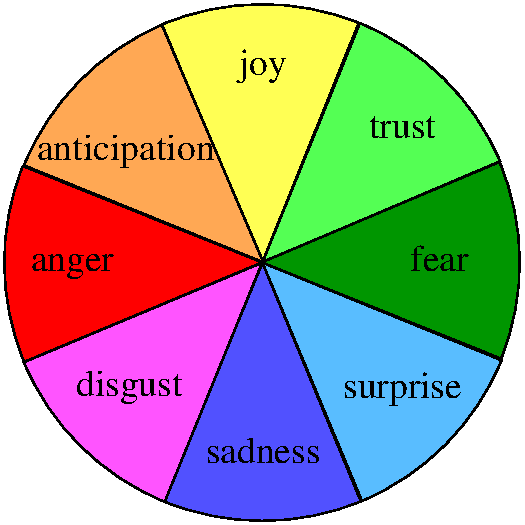
\includegraphics[width = 0.3\linewidth]{figure/plutchikWheel.pdf}
    \caption{Plutchik basic emotions}
    \label{fig:plutchikLabel}
\end{figure}

\begin{align}
    \forall \vec{C} \in \mathbf{D}, \hspace{10pt} \vec{C} &= \begin{bmatrix}
                                                e_{1} \\
                                                e_{2} \\
                                                \vdots \\
                                                e_{8}
                                                \end{bmatrix}, 
    e \in [0, 1]
\end{align}
\noindent Given the context of a story, i.e., all previous sentences $\vec{X} = \{x_1, x_2, x_3, \dots, x_m\}$, the goal is to predict the emotions $\vec{C_i}$ that will appear in the next sentence. 


Essentially, the model provides the confidence level of each categories $\mathcal{P}(\vec{C_i} | \vec{X}) = \Pi^8_{k=1}\mathcal{P}(c_k | \vec{X})$, which will be transformed into the final result by setting the threshold value to $0.600$. 

For example, for the following input sequence of sentence $\textsc{S}_1$ that serves as context, the model may predict the emotions in the next sentence to be \texttt{joy, anticipation,} and \texttt{trust} given the following sentenve.

\begin{center}
    \texttt{
    $\textsc{S}_1$: He was hoping this year to be tall enough for the coaster.
    }
\end{center}

%where does 17910 comes from, there is also 1680 in later sections
% \begin{figure}[h]
%     %% first three subfigures
%     \subfigure[Total/Avg]{%
%       \label{fig:Total_scatter}%
%       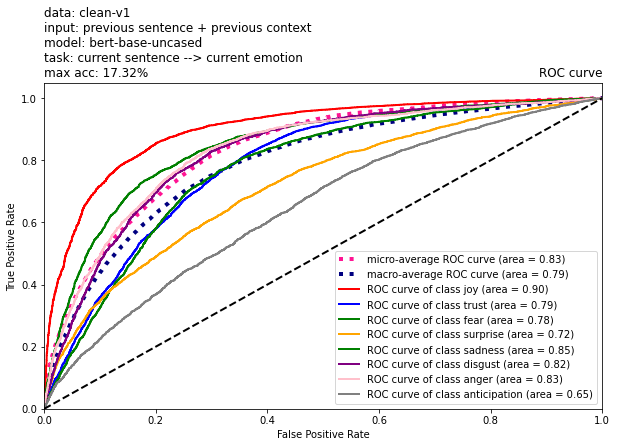
\includegraphics[width=0.31\textwidth]{figure/[ROC] curEmo-sent.png}%
%     }%
%     \hspace*{\fill}
%     \subfigure[Num/Avg]{
%       \label{fig:Num_scatter}%
%       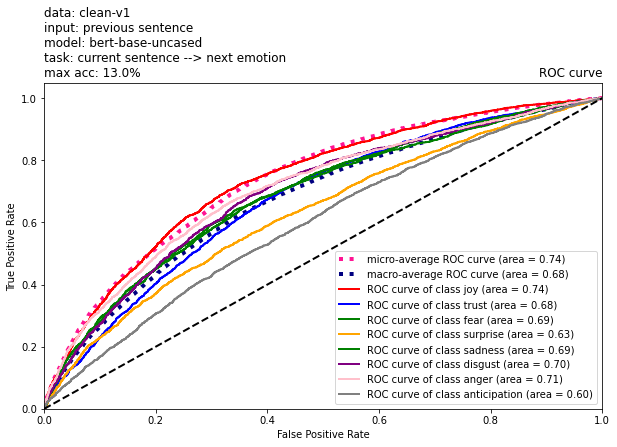
\includegraphics[width=0.31\textwidth]{figure/[ROC] nextEmo-sent.png}%
%     }%
%     \hspace*{\fill}
%     \subfigure[Raw/Avg]{
%       \label{fig:Raw_scatter}%
%       \includegraphics[width=0.31\textwidth]{images/Raw_scatter}%
%     }
    
%     %% second group of subfigures
%     \subfigure[Num/Raw]{%
%       \label{fig:Num_Raw_scatter}%
%       \includegraphics[width=0.31\textwidth]{images/Num_Raw_scatter}%
%     }%
%     \hspace*{\fill}
%     \subfigure[Total/Raw]{
%       \label{fig:Total_Raw_scatter}%
%       \includegraphics[width=0.31\textwidth]{images/Total_Raw_scatter}%
%     }%
%     \hspace*{\fill}
%     \subfigure[Num/Total]{
%       \label{fig:Num_Total_scatter}%
%       \includegraphics[width=0.31\textwidth]{images/Num_Total_scatter}%
%     }
%     \caption{Scatter plots of 6 pics.}\label{fig:Scatter}
% \end{figure}


For preparing the training data, we obtained 17,910 pairs of story context and next-sentence emotions from the Story Commonsense dataset. The dataset was divided into training and validation sets in the ratio of 6:4. We then fine-tuned the BERT$_{\textsc{Next Emo}}$ model %from Huggingface
using the task of multi-label classification. The story context is the input, and the next-sentence emotions are the output. The maximum input length of the tokenizer was set to 120. The batch size was set to 16, and the learning rate was set to $6e-6$. We ran 16 epochs for training, which took about 45 minutes on a Tesla P100-PCIE-16GB GPU. Our best model achieved a Macro ROC-AUC score of 0.69 on prediction. The prediction results are not perfect. However, they are only used as suggestions, and the user can always overwrite them. 

\subsection{Keywords Extraction}
For training the model and evaluation, we extract keywords from the original five-sentence stories. We used the \texttt{SceneGraphParser()} from~\cite{wu2019unified} to parse sentences (in natural language) into scene graphs. The entities in the scene graphs become the keywords. For example, for the following sentence: 
\begin{center}
    \texttt{
    $\textsc{S}_1$: I brought the movie home and watched the whole thing.
    }
\end{center}
We are expected to generate the following result:
\begin{center}
    \texttt{'I, the movie, the whole thing'}
\end{center}

\section{Evaluation \& Results}
% We have currently finishing fine-tuing the Teacher Network based on \texttt{Davinci-003}. It is able to provide decent results with qualified performance in various metrics including BLEU and BERT score. As further parameter-tuning is necessary, further results and visualization will be provided in the formal respot.
In this section, we present the experimental results of our creative story generation framework using Large Language Models (LLMs), between the baseline model(Zero-shot \texttt{T5$_{base}$}) and the student model with knowledge distilation from \texttt{OPT 1.3b}. We compare our approach to a baseline model fine-tuned solely based on the existing story. Both our method and the baseline use the same scale of T5 and adapt the inputs to the prompt format used in the corresponding fine-tuning phase.

In order to obtain the validity of the prompts we added to the input, we used the average of BLEU~\cite{lin-och-2004-orange} scores with n-grams ranging from 1 to 4 and BERT-scores~\cite{https://doi.org/10.48550/arxiv.1904.09675} as basic metrics in our evaluation. In addition, we use METEOR~\cite{banarjee2005} and SacreBLEU\cite{post-2018-call} as supplements to compensate for the lack of stemming and synonym matching, as well as standard exact word matching, when comparing the generated content with the ground truth.

We present the experimental results in Figure~\ref{metricCompare-baseline} and find that, compared to the baseline model, which relies solely on story context for inference, our pipeline shows consistent improvements in all metrics under the same model by introducing emotions and keywords as prompts and knowledge distillation from LLM.

The experiment results indicate that our creative story generation framework using Large Language Models (LLMs), such as T5, has shown significant improvements compared to the baseline model. By leveraging the knowledge distillation technique, we can reduce the computational overhead while maintaining high-quality text generation. Additionally, the emotion annotation generation and keywords extraction components contribute to the overall improvement of story generation quality. When comparing our framework to the baseline model, which relies solely on story context for inference, our pipeline shows consistent improvements in all metrics, such as BLEU, BERT-score, METEOR, and SacreBLEU. Overall, our experiment results suggest that our research project's methodology, which combines LLM fine-tuning, and knowledge distillation is effective in developing a robust and efficient framework for creative story generation.

\begin{figure}[h]
    \centering
    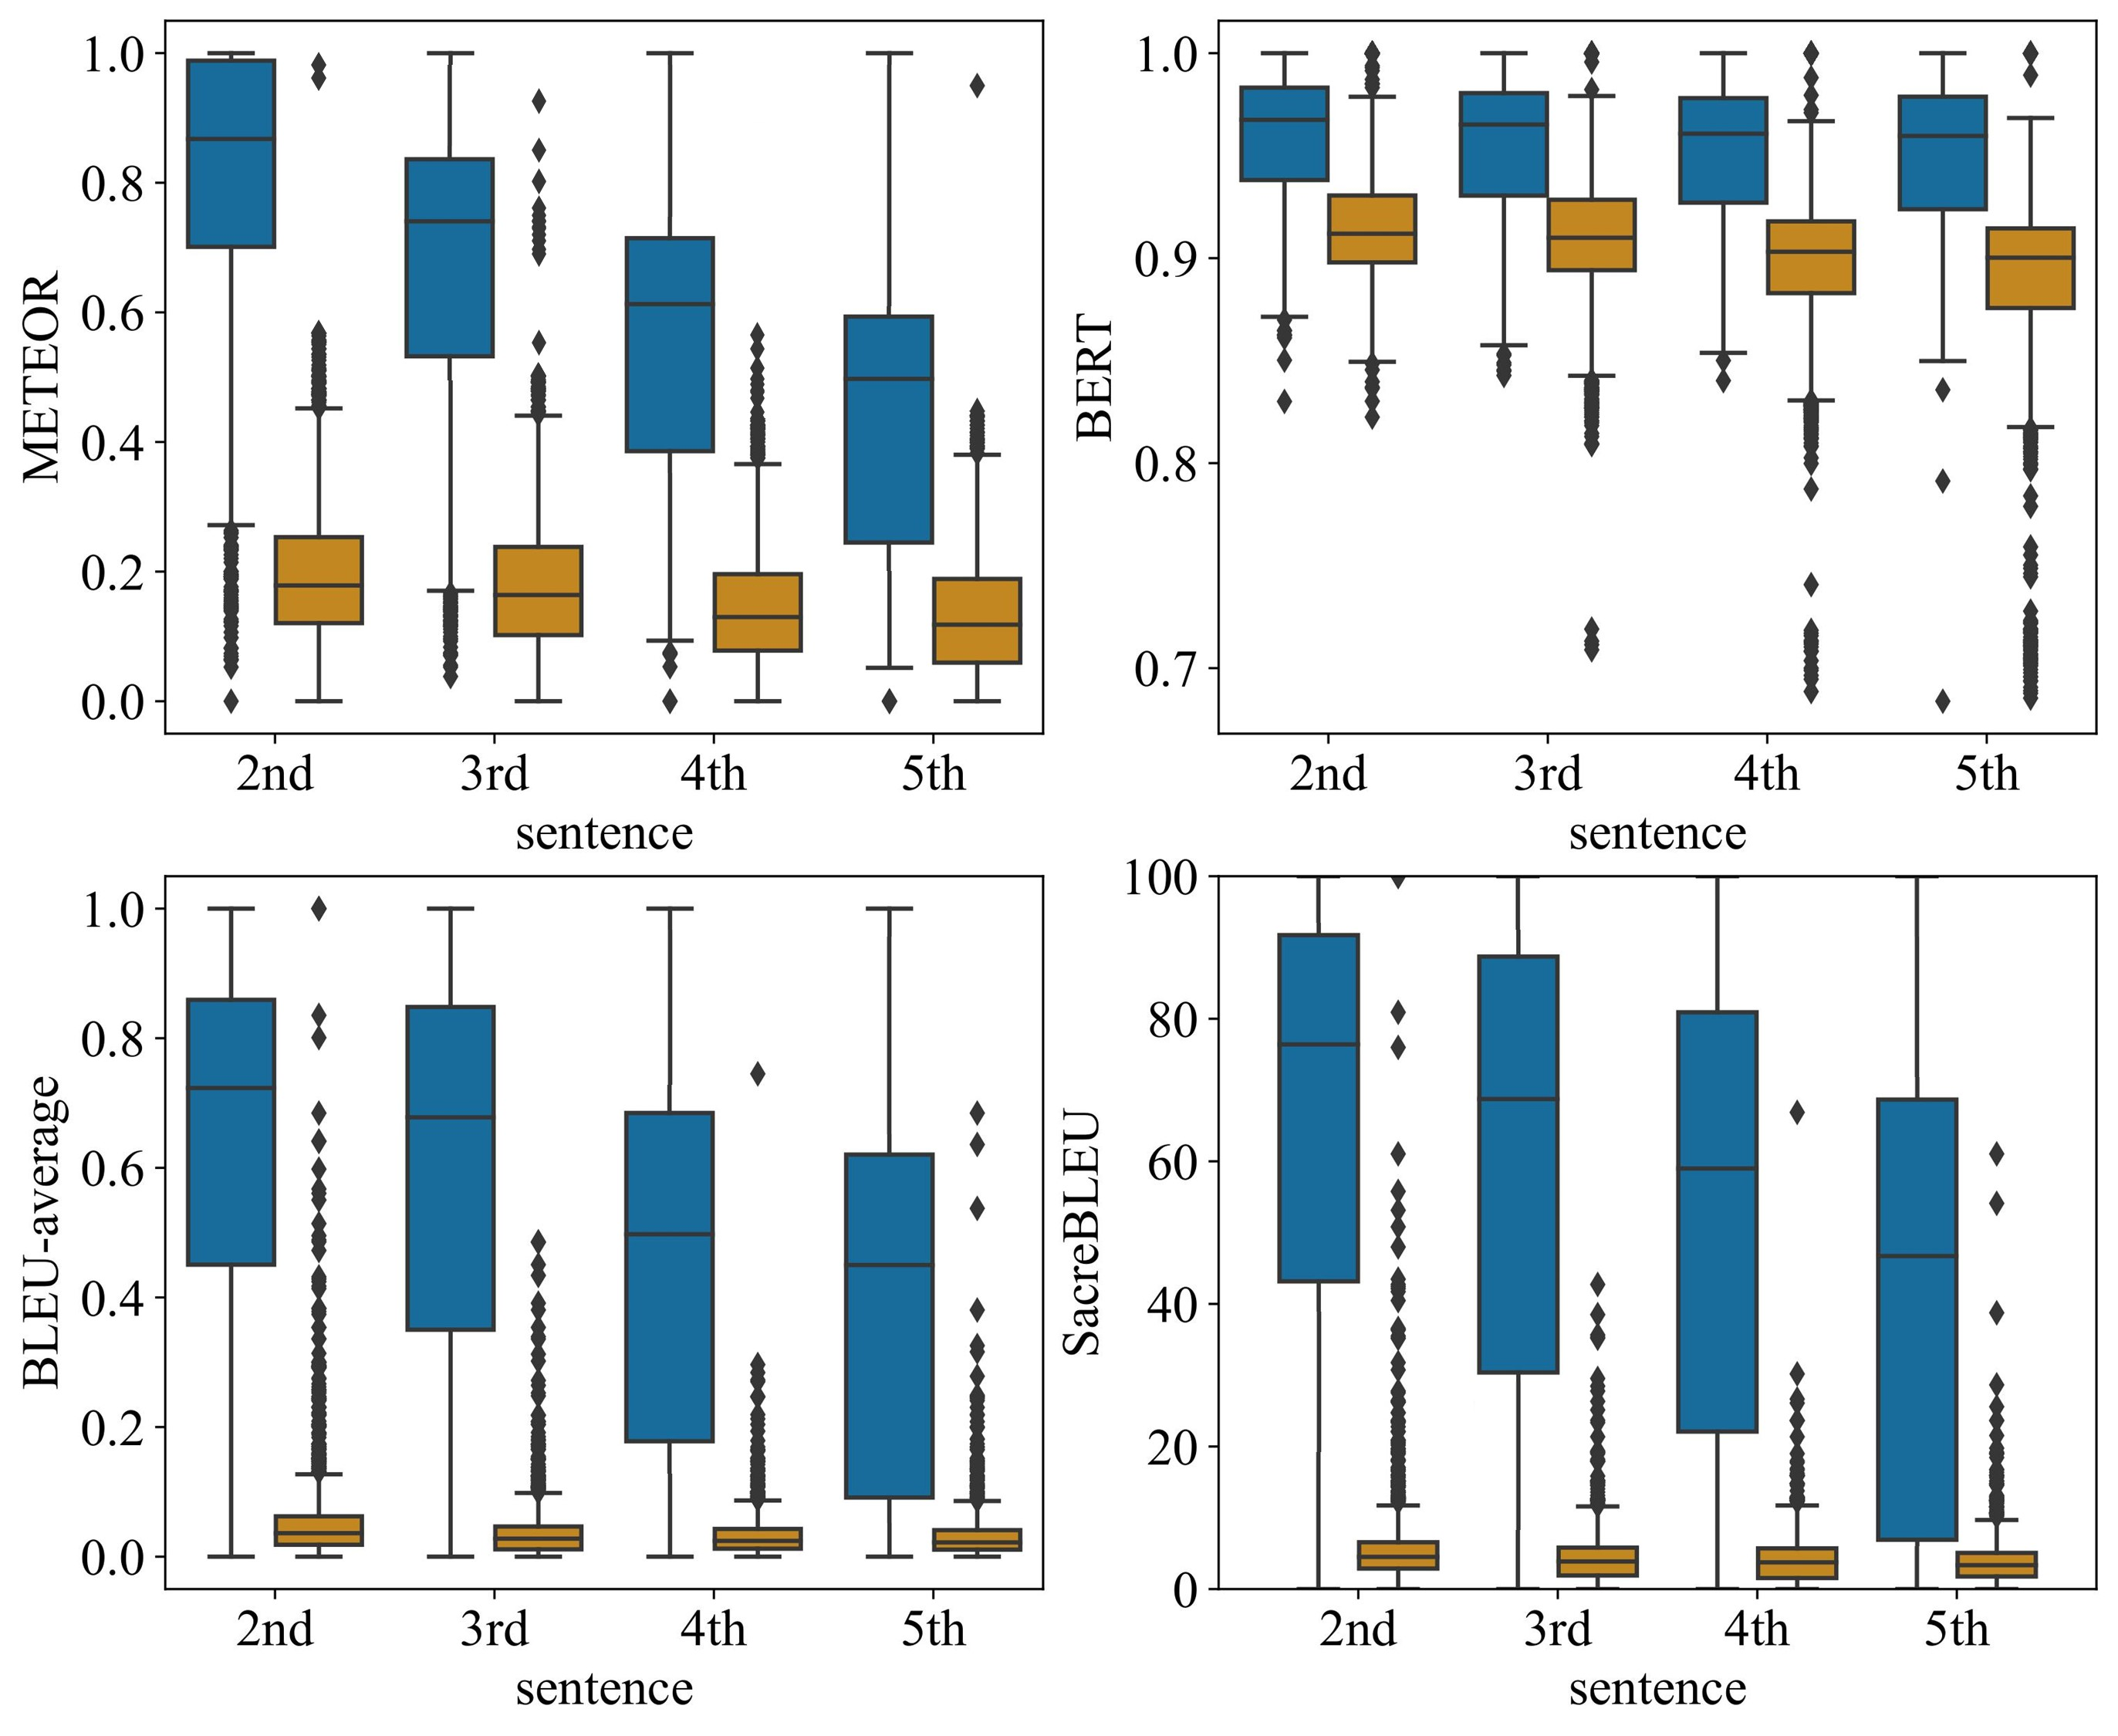
\includegraphics[width = 0.6\linewidth]{figure/RESULT_1.jpg}
    \caption{Performance distribution of the baseline model and the prompt-optimized model in 3,748 sets of experiments under different metrics The blue box on the left side of each figure represents our method, and the orange on the right side represents the baseline model.}
    \label{metricCompare-baseline}
\end{figure}

\section{Future Work}
\subsection{Replacing KL Divergence with Jensen-Shannon Divergence}
In the current implementation of knowledge distillation, the Kullback-Leibler (KL) divergence is used as a measure of the difference between the teacher and student model's probability distributions. However, there are several reasons to consider using the Jensen-Shannon (JS) divergence as an alternative in future work.

The Jensen-Shannon divergence is a symmetric measure of the difference between two probability distributions, which is derived from the KL divergence. It is defined as follows:

\begin{equation}
\text{JS}(P, Q) = \frac{1}{2} \text{KL}(P || M) + \frac{1}{2} \text{KL}(Q || M)
\end{equation}

where $P$ and $Q$ are the probability distributions being compared, and $M$ is the average of $P$ and $Q$: $M = \frac{1}{2}(P + Q)$. The JS divergence has several advantages over the KL divergence:
\begin{itemize}
    \item \textbf{Symmetry:} JS divergence is symmetric, meaning that $\text{JS}(P, Q) = \text{JS}(Q, P)$. In contrast, KL divergence is not symmetric, which may result in different outcomes when the order of the teacher and student model's probability distributions is reversed. Symmetry is an attractive property when comparing probability distributions, as it ensures that the distance measure is consistent regardless of the order in which the distributions are considered.
    \item \textbf{Finite values:} JS divergence is guaranteed to produce finite values even when the support of the two probability distributions does not overlap. In contrast, the KL divergence can produce infinite values when the distributions have non-overlapping supports. Using JS divergence can lead to a more stable optimization process, as it avoids the possibility of encountering infinite values during training.
    \item \textbf{Smoothness:} JS divergence is smoother than KL divergence, meaning that it is less sensitive to small differences between the probability distributions. This can make the optimization process more robust to noise and local minima in the loss landscape.
\end{itemize}

\subsection{Exploring Self-Distillation for Language Generation}
Another perspective for future work is exploring self-distillation~\cite{zhang2019teacher} in the context of language generation. Self-distillation involves training a model on its own output, essentially using the same model architecture for both the teacher and student models. This approach has shown promising results in various tasks, including image classification and natural language processing, and could be applied to language generation as well.

There are several potential benefits of using self-distillation for language generation:
\begin{itemize}
    \item \textbf{Regularization:} Self-distillation can act as a form of regularization, as it encourages the model to learn a smoother probability distribution over the output tokens. This can lead to better generalization performance and reduce the risk of overfitting.

    \item \textbf{Model Refinement:} By repeatedly distilling the model using its own output, it is possible to refine the model's understanding of the training data and improve its overall performance. This iterative process can help the model learn more nuanced relationships between input tokens and their corresponding output sequences.

    \item \textbf{Simplification of Implementation:} In self-distillation, both the teacher and student models have the same architecture, which simplifies the implementation process. This also reduces the computational overhead associated with maintaining two separate models during training.
\end{itemize}
\section{Conclusion}
In this paper, we have explored the potential of Large Language Models (LLMs) for creative story generation by combining LLM fine-tuning with knowledge distillation techniques. Our research project sought to develop a framework that generates coherent and engaging stories, characterized by rich narrative structures such as character development, plot progression, and conflict resolution. By utilizing both teacher and student models, we aimed to create a more computationally efficient framework capable of generating captivating stories without sacrificing the quality of the generated text.

The methodology we employed consisted of two key components: LLM fine-tuning and knowledge distillation. These components were designed to work in tandem to create an effective framework for story generation. We demonstrated the implementation of knowledge distillation using a teacher model and a student model, and discussed the equations, objective/loss function, and necessary derivations for this implementation. Our experiments showcased the potential of the proposed framework in generating creative stories, offering valuable insights for future research in this area.

In addition to the current implementation, we have identified several areas for future work, including the exploration of alternative divergence measures such as Jensen-Shannon divergence, and the investigation of self-distillation for language generation. By considering these potential improvements, we believe that our framework can be further refined, paving the way for more advanced and efficient story generation systems. Ultimately, the combination of LLMs with innovative techniques for narrative structure generation holds great promise for the future of creative storytelling in the age of artificial intelligence.

% We have used T5 as the pre-trained LLM for our story generation framework. We will explore different techniques for generating narrative structures, such as using knowledge graphs to represent characters and plot elements and controlling the generation process to ensure coherence and consistency. We will also use a fine-tuning approach to adapt the LLM to the task of story generation and improve its performance in generating coherent and engaging stories. Through this process we will derive equations in the knowledge distillation which could have an impact on the framework. We are still determining how we will implement and utilize knowledge distillation graphs.

% We expect to develop a framework that can generate coherent and engaging stories with rich narrative structures, including character development, plot progression, and conflict resolution. We also anticipate that our framework will be able to generate stories that are engaging and can be enjoyed by a wide audience. Furthermore, we expect to identify the most effective techniques for narrative structure generation and fine-tuning the LLM for story generation. \\

% \section{Conclusion}
% % Should include future work

% \section{Acknowledgements}
% We want to thank Yuetian's prior research ...

\bibliography{iclr2021_conference}
\bibliographystyle{iclr2021_conference}

\newpage
\appendix
\section{Appendix}
\begin{figure}[!htbp]
\begin{center}
    \begin{subfigure}
        \centering
        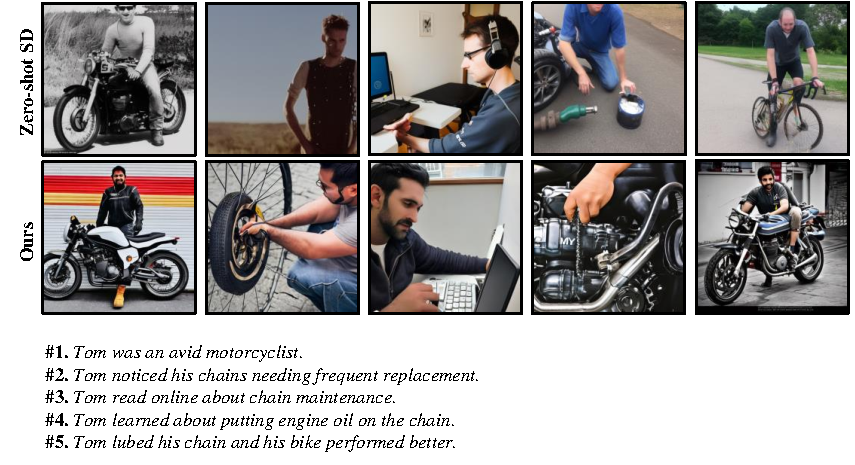
\includegraphics[width=0.76\linewidth]{figure/3-example.pdf}
        \caption*{}
    \end{subfigure}
    
    \begin{subfigure}
        \centering
        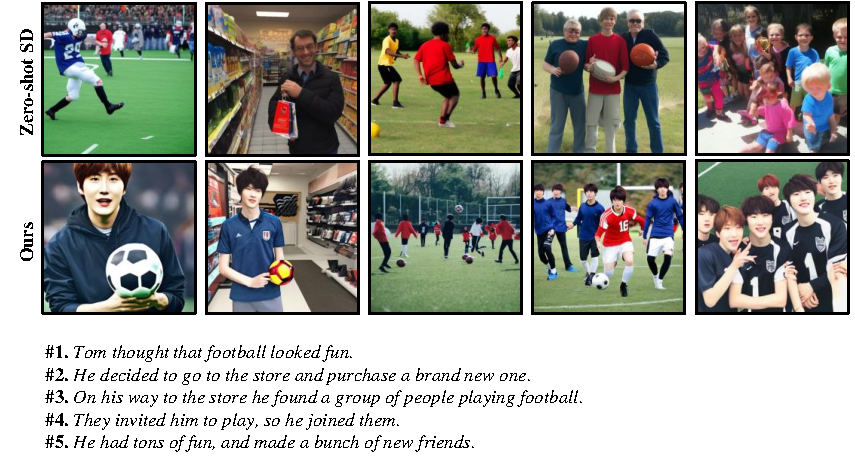
\includegraphics[width=0.76\linewidth]{figure/4-example.pdf}
        \caption*{}
    \end{subfigure}
    
    \begin{subfigure}
        \centering
        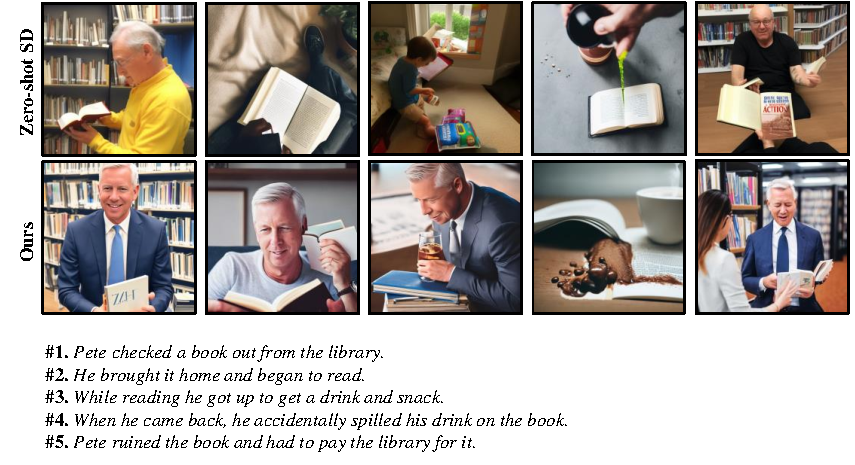
\includegraphics[width=0.76\linewidth]{figure/5-example.pdf}
        \caption*{}
    \end{subfigure}
\end{center}
    \caption{Sample generation results combined with the reseults from image generation pipeline introduced in previous work. By applying DreamBooth with name entity identification and extraction, we align the generation quality of two pipelines in terms of character consistency.}
    \label{fig:plutchikLabel}
\end{figure}

\begin{figure}[h]
    \centering
    \subfigure{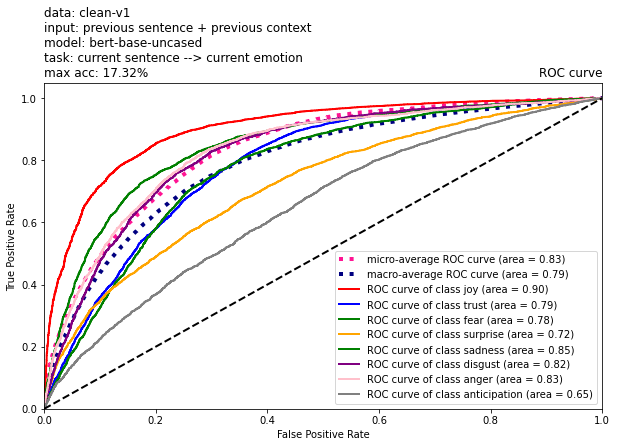
\includegraphics[width=0.48\textwidth]{figure/[ROC] curEmo-sent.png}}
    \subfigure{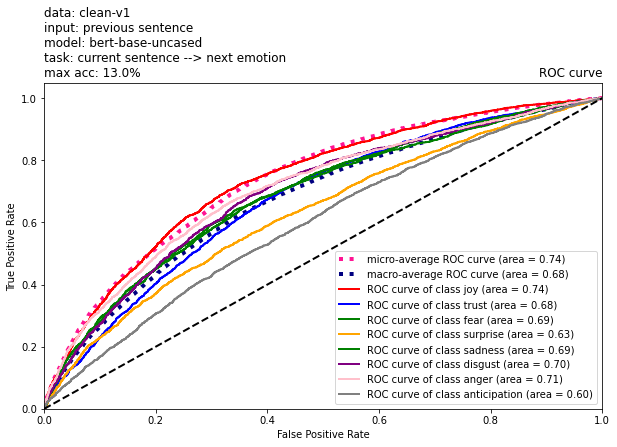
\includegraphics[width=0.48\textwidth]{figure/[ROC] nextEmo-sent.png}}
    \vspace{0.2in}
    \subfigure{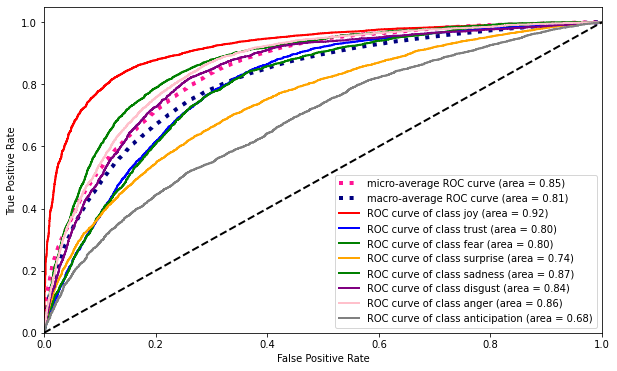
\includegraphics[width=0.48\textwidth]{figure/[ROC] curEmo-sent-notitle.png}}
    \subfigure{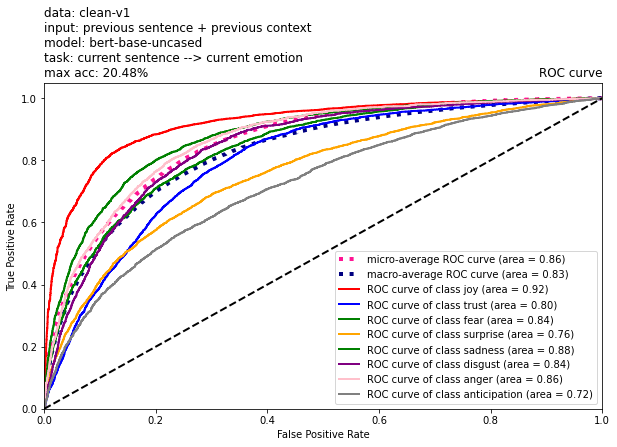
\includegraphics[width=0.48\textwidth]{figure/[ROC] curEmo-sent+context.png}}
    \vspace{0.2in}
    \subfigure{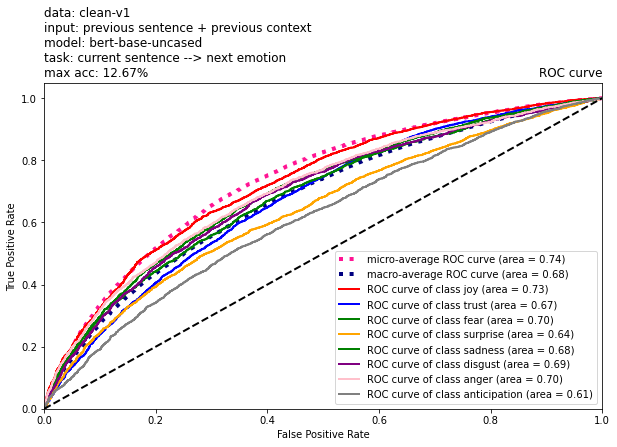
\includegraphics[width=0.48\textwidth]{figure/[ROC] nextEmo-sent+context.png}}
    \subfigure{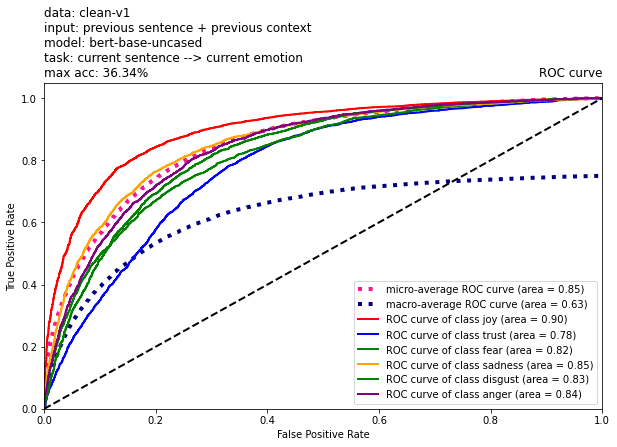
\includegraphics[width=0.48\textwidth]{figure/[ROC] curEmo-sent+context-remSurAni.png}}
    \caption{All ROC visualization for each emotion label result under different emotion suggester settings}
\end{figure}


\end{document}
